\chapter{Objectives and Criteria}
\section{Detailed Task Description}
The goal of the thesis is to add value to real business documents by aggregating expenses into clusters of similar expenses. The supplied document dataset consists of 150.000 invoices. The invoices contain different information, for example the vendor, billing amount or a description of the goods. Valuable information for companies would be insight into the different categories of expenses and the corresponding cost. With traditional data analysis methods, the company’s controlling departments cannot identify which expenses are similar in nature (for example logistics costs). 

The task is to perform a full data analysis on the supplied dataset. The dataset is to be prepared for processing with established methods. An evaluation for different means of feature extraction, machine learning, model evaluation and visualization should be performed. With the evaluation a complete flow for the data processing should be presented. The result should be an added value to the dataset in the form of aggregated expenses.

\section{Criteria set by SAP SE}
none?

\section{Research Model}
To solve the task described in chapter 1.2, this paper employs the \ac{CRISP-DM} \cite{CRISPDM2000}. This model puts forward a structure for conducting data mining projects. \ac{CRISP-DM} was developed in 1996 by three companies, which are now the partners of the \ac{CRISP-DM} consortium: NCR, DaimlerChrysler AG and SPSS Inc. 

\begin{figure}[ht]
	\centering
	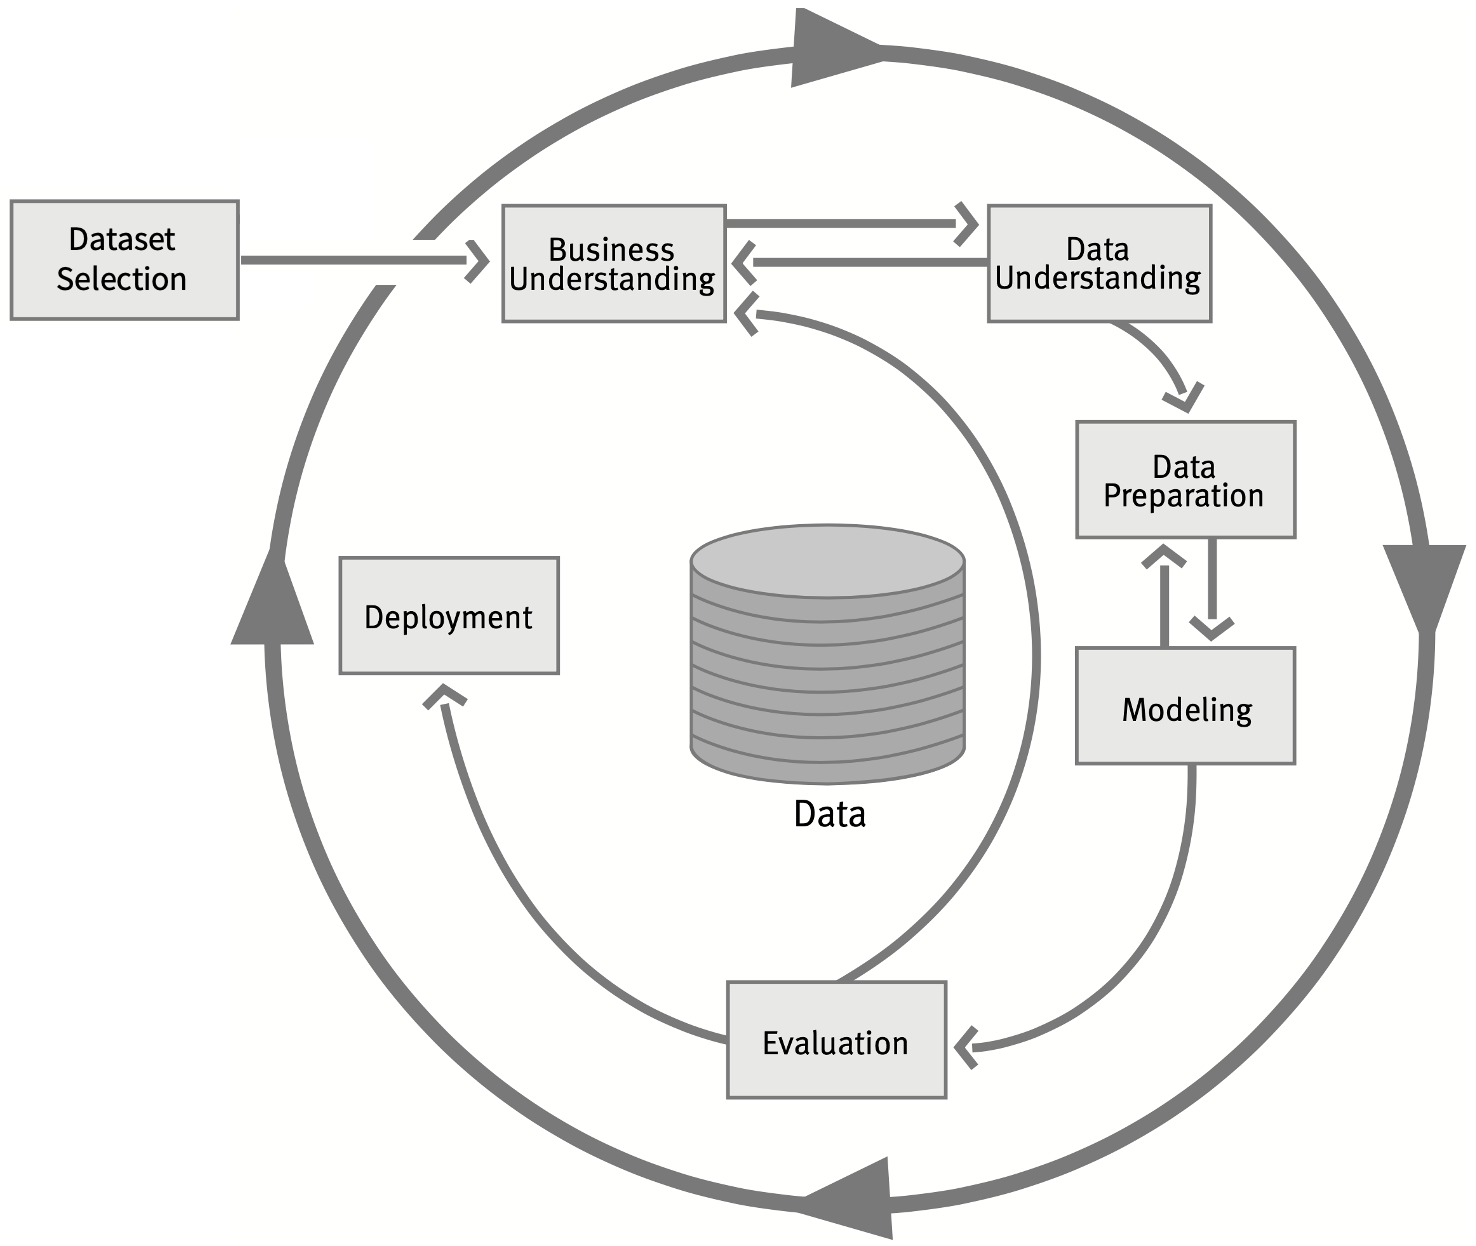
\includegraphics[height=10cm]{Bilder/Research_Model.png}
	\caption{Adjusted CRISP-DM Model}
	\label{fig:CRISM-DM}
\end{figure}

Classically, the reference model consists of six phases: Business Understanding, Data Understanding, Data Preparation, Modeling, Evaluation, and Deployment. For this thesis the model was adapted to reflect all tasks encompassed. The phase "Dataset Selection" was added, resulting in a total of seven phases.

Fundamentally, the \ac{CRISP-DM} model is of circular nature, reflecting the fact that data science projects underly the premise of continuous improvement. After the deployment of one solution, monitoring can give insights which allow for deeper business understanding, triggering the start of a new circuit of the model.




- what does the model describe?

- what are the steps?

- why do I use this model?

- Which alterations were made?
 